%!TEX root=../paper.tex

\section{Implementation}
Polite is implemented on top of Pharo Smalltalk and PetitParser is used to define its grammar using parsing expressions. The implementation can be found online. The code examples from this paper are fragments of a larger example that can also be found in the Polite image available online. 

\begin{figure}[h]
	\centering
	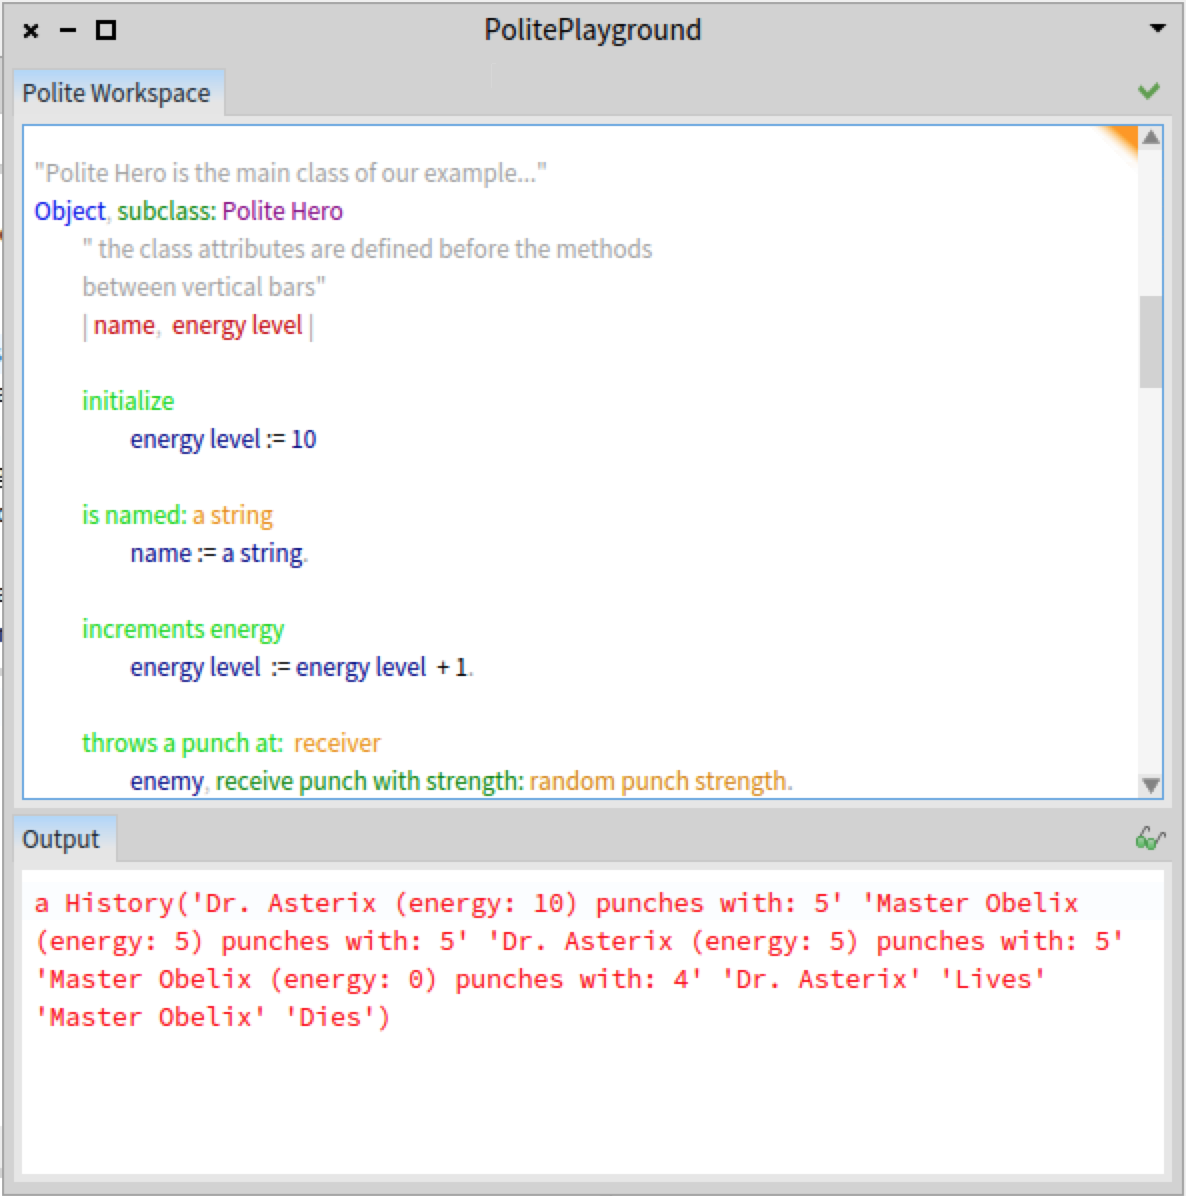
\includegraphics[width=0.5\textwidth]{images/playground.png}
	\caption{The Polite Playground provides a syntax highlighting code editor for Polite}
	\label{fig:figure1}
\end{figure}